\documentclass[12pt]{article}

\usepackage[active]{srcltx}

\usepackage{amsmath,amsfonts,amssymb,amsthm}
\usepackage{easybmat}
\usepackage{graphicx}
%\usepackage[hypertex]{hyperref}
%\usepackage[pdftex]{hyperref}
\usepackage{fancyhdr}
\usepackage{subfigure}

\usepackage{makeidx}
\makeindex

\theoremstyle{plain}
\newtheorem{theorem}{Theorem}
\newtheorem{property}[theorem]{Property}
\newtheorem{condition}[theorem]{Condition}
\newtheorem{proposition}[theorem]{Proposition}
\newtheorem{axiom}[theorem]{Axiom}
\newtheorem{lemma}[theorem]{Lemma}
\newtheorem{corollary}[theorem]{Corollary}
%%
% % Make numbering specific to the Appendix
% \newtheorem{Atheorem}{Theorem}[chapter]
% \newtheorem{Aproperty}[Atheorem]{Property}
% \newtheorem{Acondition}[Atheorem]{Condition}
% \newtheorem{Aproposition}[Atheorem]{Proposition}
% \newtheorem{Aaxiom}[Atheorem]{Axiom}
% \newtheorem{Alemma}[Atheorem]{Lemma}
% \newtheorem{Acorollary}[theorem]{Corollary}

% Make definitions non italicized
%\theoremstyle{definition}
\newtheorem{definition}[theorem]{Definition}
% Make numbering specific to the Appendix
%\newtheorem{Adefinition}[Atheorem]{Definition}
\newenvironment{defi}{\vskip0.2cm\addtocounter{theorem}{1}\par\noindent\bf Definition~\arabic{section}.\arabic{subsection}.\arabic{theorem}\rm.}{\hfill{$\circ$}\par\vskip0.25cm}


%% Example environment and counter.
\newcounter{cmpt_exercise}
\newenvironment{exercise}{\addtocounter{cmpt_exercise}{1}\vskip0.2cm\par\noindent\begin{small}\bf Exercise~\arabic{cmpt_exercise}\,\,\rm --}{\hfill{$\circ$}\end{small}\par\vskip0.25cm}
\newenvironment{problem}{\addtocounter{cmpt_exercise}{1}\vskip0.2cm\par\noindent{\Large\bf Problem~\arabic{cmpt_exercise}\,\,\rm --}}{\par\vskip0.25cm}


\newenvironment{example}{\vskip0.2cm\par\noindent\begin{small}\bf Example\,\,\rm --}{\hfill{$\diamond$}\end{small}\par\vskip0.25cm}
\newenvironment{remark}{\vskip0.2cm\par\noindent\begin{small}\bf Remark\,\,\rm --}{\hfill{$\circ$}\end{small}\par\vskip0.25cm}
%\newenvironment{aparte}[1]{\vskip0.2cm\par\noindent\begin{quote}\begin{small}\bf Apart\'e : #1\,\,\rm --}{\hfill{$\circ$}\end{small}\end{quote}\par\vskip0.25cm}
\newenvironment{aparte}[1]{\vskip0.3cm\par\begin{center}\begin{tabular}{|p{0.9\textwidth}|}\hline{\bf Apart\'e : #1}}{\\ \hline\end{tabular}\end{center}\par\vskip0.25cm}

\renewcommand{\labelenumi}{\roman{enumi})}
\renewcommand{\labelenumii}{\alph{enumii})}
\newcommand{\espv}{\vspace{.5\baselineskip}}
\def\IR{\mathbb{R}}
\def\IC{\mathbb{C}}
\def\IN{\mathbb{N}}
\def\IQ{\mathbb{Q}}
\def\IZ{\mathbb{Z}}
\def\rank{\textrm{rank }}
\def\Sp{\textrm{Sp }}
\def\Span{\textrm{Span }}
\def\Tr{\textrm{Tr }}
\def\D{\mathcal{D}}
\def\I{\mathcal{I}}
\def\U{\mathcal{U}}
\def\R{\mathcal{R}}
\def\Q{\mathcal{Q}}
\def\O{\mathcal{O}}
\def\Mn{\mathcal{M}_n}
\def\NN#1{\|#1\|}
\def\N3#1{|\!|\!|#1|\!|\!|}
\def\diag{\textrm{diag}}
\def\tr{\textrm{tr}}
\def\ker{\textrm{Ker }}

\def\M{\mathcal{M}}

\setlength{\textwidth}{17cm} 
\addtolength{\oddsidemargin}{-1.5cm}
\setlength{\textheight}{22cm}
\addtolength{\topmargin}{-2cm} 
\setlength{\headheight}{25.3pt}

%% Fancyhdr related stuff
\pagestyle{fancy}
\lhead{MATH 3820 -- Intro Math Modelling -- Assignment 1}
\rhead{\thepage}
\cfoot{}

\usepackage[hang,small,bf]{caption2}
\setlength{\captionmargin}{20pt}

\makeatletter
\def\cleardoublepage{\clearpage\if@twoside \ifodd\c@page\else
\hbox{}
% \vspace*{\fill}
% \begin{center}
% This page intentionally contains only this sentence.
% \end{center}% Make numbering specific to the Appendix
\newtheorem{Atheorem}{Theorem}[chapter]
\newtheorem{Aproperty}[Atheorem]{Property}
\newtheorem{Acondition}[Atheorem]{Condition}
\newtheorem{Aproposition}[Atheorem]{Proposition}
\newtheorem{Aaxiom}[Atheorem]{Axiom}
\newtheorem{Alemma}[Atheorem]{Lemma}
\newtheorem{Acorollary}[theorem]{Corollary}

% \vspace{\fill}
\thispagestyle{empty}
\newpage
\if@twocolumn\hbox{}\newpage\fi\fi\fi}
\makeatother

%\author{Julien Arino}
%\address{University of Manitoba}
%\title{MATH 8430\\ Lecture Notes}
\title{University of Manitoba\\ Math 38200 -- Winter 2007}
\author{Assignment 1}
\date{Solutions}

\renewcommand{\abstractname}{Instructions}
%%%%%%%%%%%%%%%%
%%%%%%%%%%%%%%%%
%%%%%%%%%%%%%%%%
%%%%%%%%%%%%%%%%
%%%%%%%%%%%%%%%%
%%%%%%%%%%%%%%%%
\begin{document}

\maketitle

\vskip1cm
\noindent
The Ricker model of growth of a single population takes the form
\begin{equation}\label{eq:Ricker}
N_{t+1}=N_t e^{r\left(1-\frac{N_t}K\right)},
\end{equation}
with $r,K>0$ and initial condition $N_0>0$.

\vskip1cm
\noindent
{\bf 1. (5 points)} 
Setting $x_t=N_t/K$ is similar to saying that $N_t=Kx_t$. Substituting this value into \eqref{eq:Ricker}, we get
\begin{align*}
Kx_{t+1} &= Kx_t e^{r\left(1-\frac{Kx_t}K\right)} \\
&= Kx_t e^{r(1-x_t)},
\end{align*}
and therefore,
\begin{equation}\label{eq:Ricker_dimless}
x_{t+1}=x_t e^{r(1-x_t)}.
\end{equation}
Note that $N$ has units \emph{number of individuals}, $K$ has units \emph{number of individuals}, and therefore $N/K$ is dimensionless.

\vskip0.4cm
\noindent
{\bf 2. (5 points)} 
Suppose that $x_0>0$. Then $x_1>0$, since $e^{r(1-x_0)}>0$ and $x_0>0$. Now suppose that $x_k>0$. Then $x_{k+1}>0$, since $e^{r(1-x_k)}>0$ and $x_k>0$. Therefore, by induction, $x_t>0$ for all $t$.

\vskip0.4cm
\noindent
{\bf 3. (15 points)} 
We set
\[
f(x)=xe^{r(1-x)}
\]
and seek $p$ such that $p=f(p)$. We have
\begin{align*}
p=f(p) &\Leftrightarrow p=pe^{r(1-p)} \\
&\Leftrightarrow p=0\textrm{ or }1=e^{r(1-p)} \\
&\Leftrightarrow p=0\textrm{ or }0=r(1-p)\qquad\textrm{(taking the $\ln$ of both sides)} \\
&\Leftrightarrow p=0\textrm{ or }p=1.
\end{align*}
So there are two fixed points, $0$ and $1$. To study the stability, we compute
\[
f'(x)=(1-rx)e^{r(1-x)}.
\]
Then
\[
|f'(0)|=|e^r|=e^r,
\]
so that $0$ is attracting if $r>0$ and repelling if $r<0$. Since it is assumed that $r>0$, $0$ is always attracting.
Also,
\[
|f'(1)|=|1-r|.
\]
So
\begin{align*}
|f'(1)|<1 &\Leftrightarrow |1-r|<1 \\
&\Leftrightarrow -1<1-r<1 \\
&\Leftrightarrow -2<-r<0 \\
&\Leftrightarrow 0<r<2.
\end{align*}
Therefore, if $0<r<2$, $1$ is attracting, and if $r>2$, $1$ is repelling.

\vskip0.4cm
\noindent
{\bf 4. (10 points)} 
We have
\begin{align*}
f^2(x) &= f(f(x)) \\
&= f(x)e^{r(1-f(x))} \\
&= xe^{r(1-x)}e^{r(1-xe^{r(1-x)})}
\end{align*}
We have a period 2 point if $f^2(p)=p$ for some $p$, that is,
\[
p=pe^{r(1-p)}e^{r(1-pe^{r(1-p)})}.
\]
The first conclusion is that $p=0$ is a fixed point (but since 0 is also a fixed point, it is not a point with least period 2). Supposing now that $p\neq 0$, we thus must find $p$ such that
\[
1=e^{r(1-p)}e^{r(1-pe^{r(1-p)})}.
\]
Taking the $\ln$ of both sides of the equation, we have
\[
0=r(1-p)+r\left(1-pe^{r(1-p)}\right).
\]
Note that it is clear from this equation that $p=1$ is a fixed point of $f^2$, that is, a period 2 point (but, as for $p=0$, it is not a point with least period 2, since $p=1$ is also a fixed point).
Therefore, 
\[
-r(1-p)=r(1-pe^{r(1-p)}),
\]
that is,
\[
p\left(e^{r(1-p)}+1\right)-2=0.
\]
Let us define
\[
\Gamma(p)=p\left(e^{r(1-p)}+1\right)-2.
\]
We have $\Gamma(0)=-2$, and $\lim_{p\to\infty}\Gamma(p)=\infty$, therefore, since $\Gamma$ is continuous, it must have at least one root. Clearly, $p=1$ is such a root, but are there others?
We have
\[
\Gamma'(p)=1+(1-rp)e^{r(1-p)}
\]
and
\[
\Gamma''(p)=-r(2-rp)e^{r(1-p)}
\]
At $0$, $\Gamma''(0)=-2re^r<0$, that is, $\Gamma$ is concave down. It then changes concavity when $rp=2$, i.e., for $p=2/r$, and then remains concave up for all values of $p>r/2$. Now note that since $0<r<2$, it follows that $1<2/r<\infty$, so that the inflection point occurs after $p=1$.

On the other hand, $\Gamma'(0)=1+e^r>0$, so $\Gamma$ is initially increasing, from the value $-2$. Putting all this together, we have that $\Gamma$ has the shape shown in Figures~\ref{fig:Gamma_1} and \ref{fig:Gamma_2}.

\begin{figure}[htbp]
\begin{center}
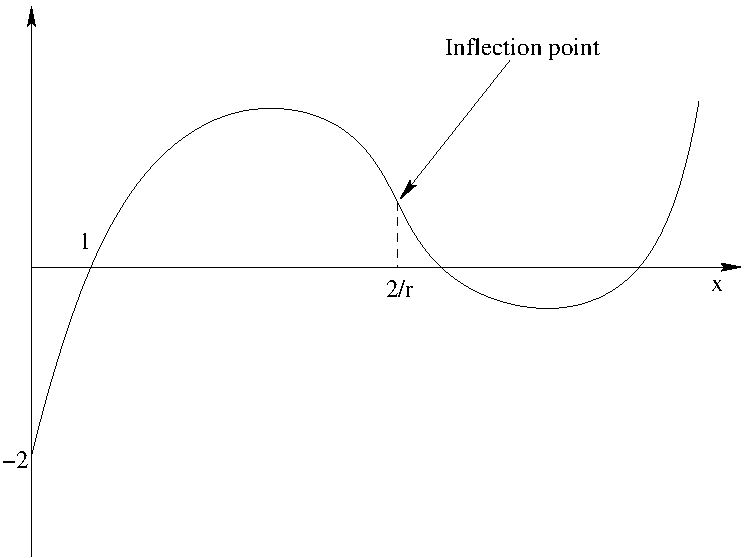
\includegraphics[width=0.45\textwidth]{fig1_a}
\caption{One possibility for $\Gamma$ that would lead to two positive period 2 points for \eqref{eq:Ricker_dimless}.}
\label{fig:Gamma_1}
\end{center}
\end{figure}


\begin{figure}[htbp]
\begin{center}
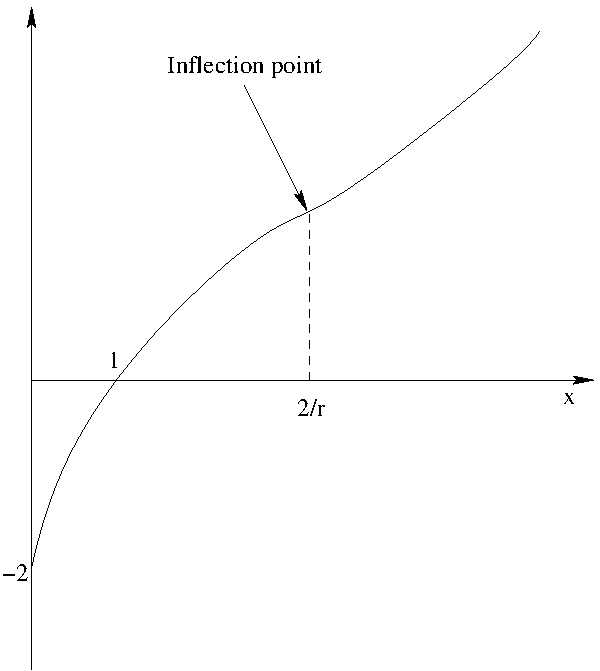
\includegraphics[width=0.45\textwidth]{fig1_b}
\caption{One possibility for $\Gamma$ that would lead to $x=1$ as a positive period 2 point for \eqref{eq:Ricker_dimless}.}
\label{fig:Gamma_2}
\end{center}
\end{figure}

To be able to exclude the possibility of the case of Figure~\ref{fig:Gamma_1} happening, we reason as follows. The main difference between Figures~\ref{fig:Gamma_1} and \eqref{fig:Gamma_2} is that when the inflection point is reached, $\Gamma$ is increasing in Figure~\ref{fig:Gamma_2}.



\vskip0.4cm
\noindent
{\bf 5.  (10 points)} 
Try to find 2-periodic points of \eqref{eq:Ricker_dimless} analytically (show your work). Then, do so using a numerical software. Under what conditions are these periodic points stable? Evaluate the stability of the points you found for a few sample values of $r$, using a numerical software.

\vskip0.4cm
\noindent
{\bf 6. (10 points)} 
Using numerical software, draw a bifurcation diagram for \eqref{eq:Ricker_dimless}, for $r$ varying in $(0,5]$. What do you observe?

\end{document}